\documentclass[aspectratio=43]{beamer}
\usepackage[english]{babel}
\usepackage{amsthm}
\usepackage{mathtools}
\usepackage{physics}
\usepackage{calligra}
\usepackage{csquotes}
\usepackage{tensor}
\usepackage[thicklines]{cancel}
\usepackage{tcolorbox}
\usepackage{pstricks}
\usepackage[backend=biber, bibstyle=nature, sorting=nty, citestyle=numeric-comp]{biblatex} %Custom bibliography
\usepackage{etoolbox}
\makeatletter
\patchcmd{\@verbatim}
{\verbatim@font}
{\verbatim@font\small}
{}{}
\makeatother
\addbibresource{bib.bib} %Load references


\DeclareMathAlphabet{\mathcalligra}{T1}{calligra}{m}{n}
\DeclareFontShape{T1}{calligra}{m}{n}{<->s*[2.2]callig15}{}
\newcommand{\scriptr}{\mathcalligra{r}\,}
\newcommand{\boldscriptr}{\pmb{\mathcalligra{r}}\,}
\def\rc{\scriptr}
\def\brc{\boldscriptr}
\def\hrc{\hat\brc}
\newcommand{\ie}{\emph{i.e.}} %id est
\newcommand{\eg}{\emph{e.g.}} %exempli gratia
\newcommand{\rtd}[1]{\ensuremath{\left\lfloor #1 \right\rfloor}}
\newcommand{\dirac}[1]{\ensuremath{\delta \left( #1 \right)}}
\newcommand{\diract}[1]{\ensuremath{\delta^3 \left( #1 \right)}}
\newcommand{\e}{\ensuremath{\epsilon_0}}
\newcommand{\m}{\ensuremath{\mu_0}}
\newcommand{\V}{\ensuremath{\mathcal{V}}}
\newcommand{\prnt}[1]{\ensuremath{\left(#1\right)}} %parentheses
\newcommand{\colch}[1]{\ensuremath{\left[#1\right]}} %square brackets
\newcommand{\chave}[1]{\ensuremath{\left\{#1\right\}}}  %curly brackets

\useoutertheme{infolines}
\useinnertheme{rectangles}
\usefonttheme{professionalfonts}


\definecolor{orange}{HTML}{f28165}
\definecolor{gray}{HTML}{303030}
\definecolor{yellow}{HTML}{f0be52}
\definecolor{lightorange}{HTML}{f19e58}

\renewcommand{\CancelColor}{\color{orange}}

\makeatletter
\newcommand{\mybox}[1]{%
	\setbox0=\hbox{#1}%
	\setlength{\@tempdima}{\dimexpr\wd0+13pt}%
	\begin{tcolorbox}[colback=orange,colframe=orange,boxrule=0.5pt,arc=4pt,
		left=6pt,right=6pt,top=6pt,bottom=6pt,boxsep=0pt,width=\@tempdima]
		\textcolor{white}{#1}
	\end{tcolorbox}
}
\makeatother

\usecolortheme[named=orange]{structure}
\usecolortheme{sidebartab}
\usecolortheme{orchid}
\usecolortheme{whale}
\setbeamercolor{alerted text}{fg=yellow}
\setbeamercolor{block title alerted}{bg=alerted text.fg!90!black}
\setbeamercolor{block title example}{bg=lightorange!60!black}
\setbeamercolor{background canvas}{bg=gray}
\setbeamercolor{normal text}{bg=gray,fg=white}

\setbeamertemplate{footline}
{
	\leavevmode%
	\hbox{%
		\begin{beamercolorbox}[wd=.333333\paperwidth,ht=2.25ex,dp=1ex,center]{author in head/foot}%
			\usebeamerfont{author in head/foot}\insertshortauthor~~(\insertshortinstitute)
		\end{beamercolorbox}%
		\begin{beamercolorbox}[wd=.333333\paperwidth,ht=2.25ex,dp=1ex,center]{title in head/foot}%
			\usebeamerfont{title in head/foot}\insertshorttitle
		\end{beamercolorbox}%
		\begin{beamercolorbox}[wd=.333333\paperwidth,ht=2.25ex,dp=1ex,center]{date in head/foot}%
			\usebeamerfont{date in head/foot}\insertframenumber/\inserttotalframenumber%\insertshortdate{}%\hspace*{2em}
			
			%#turning the next line into a comment, erases the frame numbers
			%\insertframenumber{} / \inserttotalframenumber\hspace*{2ex} 
			
	\end{beamercolorbox}}%
	\vskip0pt%
}


\setbeamertemplate{blocks}[rectangle]
\setbeamercovered{dynamic}

\setbeamertemplate{section page}
{
	\begin{centering}
		\begin{beamercolorbox}[sep=27pt,center]{part title}
			\usebeamerfont{section title}\insertsection\par
			\usebeamerfont{subsection title}\insertsubsection\par
		\end{beamercolorbox}
	\end{centering}
}

%\setbeamertemplate{subsection page}
%{
%	\begin{centering}
%		\begin{beamercolorbox}[sep=12pt,center]{part title}
%			\usebeamerfont{subsection title}\insertsubsection\par
%		\end{beamercolorbox}
%	\end{centering}
%}

\newcommand{\hlight}[1]{\colorbox{violet!50}{#1}}
\newcommand{\hlighta}[1]{\colorbox{red!50}{#1}}

\title{Challenging Final Project - Robot Server Interaction} %->->->->-> Check hyperref title <-<-<-<-<-
\subtitle{CS565 - Scientific Computing}
\author[A. Dunn \& J. Phan]{Andrew Dunn and Justin Phan}
\institute[CSCWU]{
    Department of Computer Science%
    \\%
    Central Washington University%
} %You can change the Institution if you are from somewhere else
\date{\today}
%\logo{
\includegraphics[width= 0.2\textwidth]{images/a-logo.png}}

\begin{document}
    
    \frame{\titlepage}
    
    \begin{frame}{Summary}
        \tableofcontents
    \end{frame}
    
    \section{Trigger Sentences for our Robot}
    
    \frame{\sectionpage}
    
    \begin{frame}{Sentences that will trigger the robot}
		\begin{itemize}
			\item Give me a quote
			\pause
			\item I'd like a quote
			\pause
			\item Can I have a quote
		\end{itemize}
	\end{frame}
	\begin{frame}{Nao 6}
		\begin{figure}
			\centering
			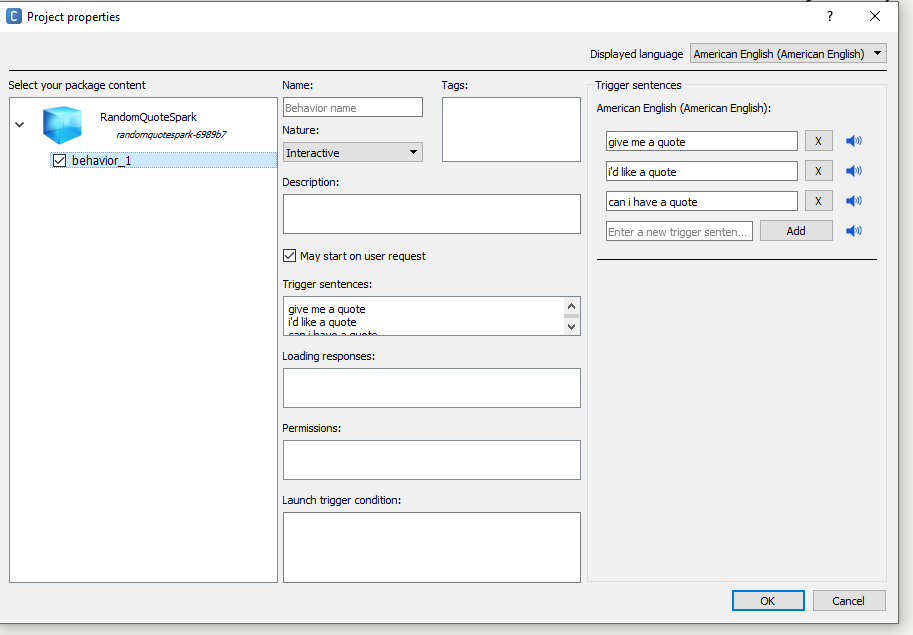
\includegraphics[width =0.7\linewidth]{robot-spark-proj/screenshot-3.PNG}
			\caption{Robot trigger}
		\end{figure}

	\end{frame} 
    
    \section{Our Code}
    
    \frame{\sectionpage}

\begin{frame}{Setting up the VPS - PHP Script}
	\centering
	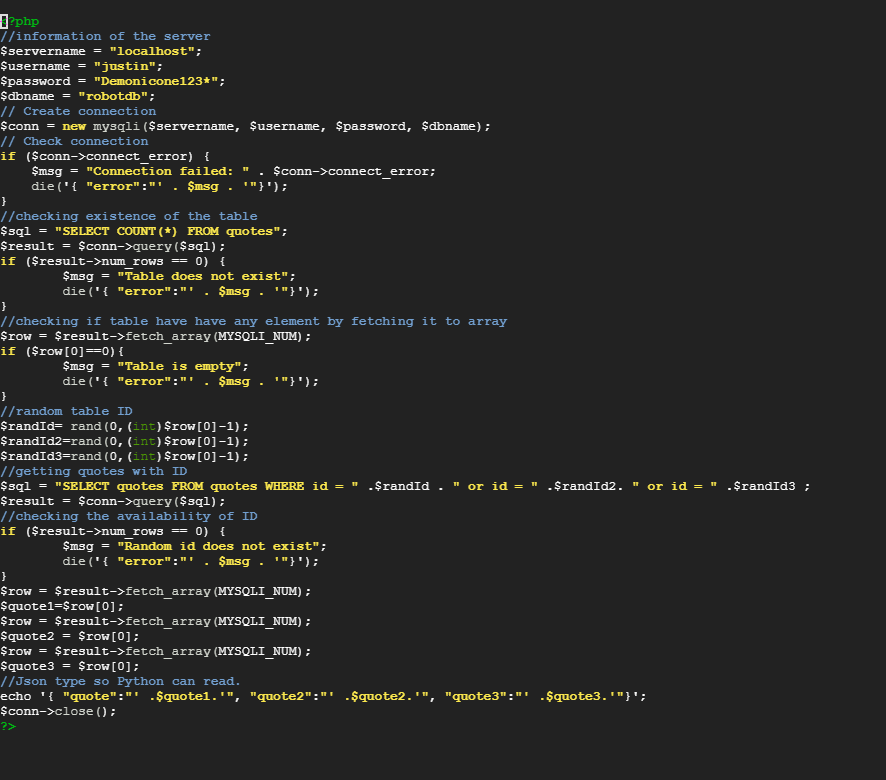
\includegraphics[width =0.7\linewidth]{images/CodeFromphpFile.PNG}
\end{frame}
\begin{frame}{Setting up the VPS - Python Example}
	\centering
	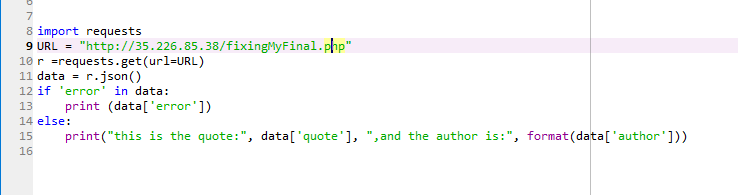
\includegraphics[width =1.1\linewidth]{images/Capture.PNG}
\end{frame}
\begin{frame}{Setting up the VPS - MariaDB}
	\centering
	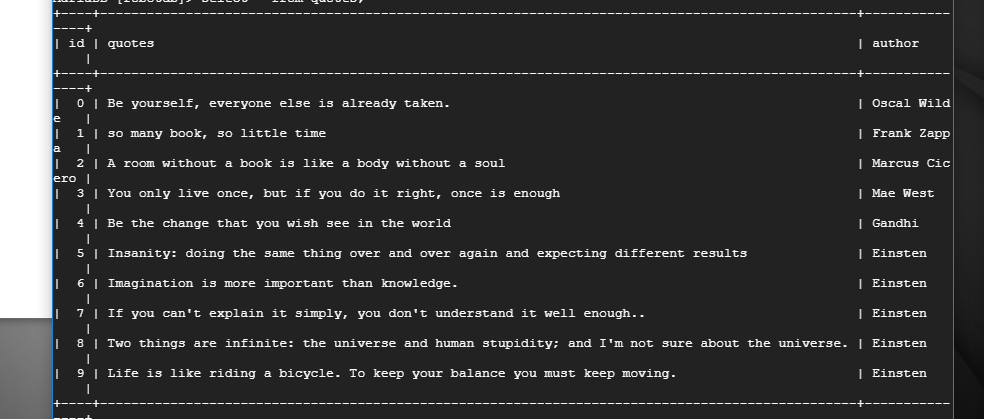
\includegraphics[width =1\linewidth]{images/tablemysql.PNG}
\end{frame}
 
    
    \section{Live Demo}
    
    \frame{\sectionpage}
    
    \begin{frame}{Robot Nao 6 Database}
    	\begin{figure}
    		\centering
    		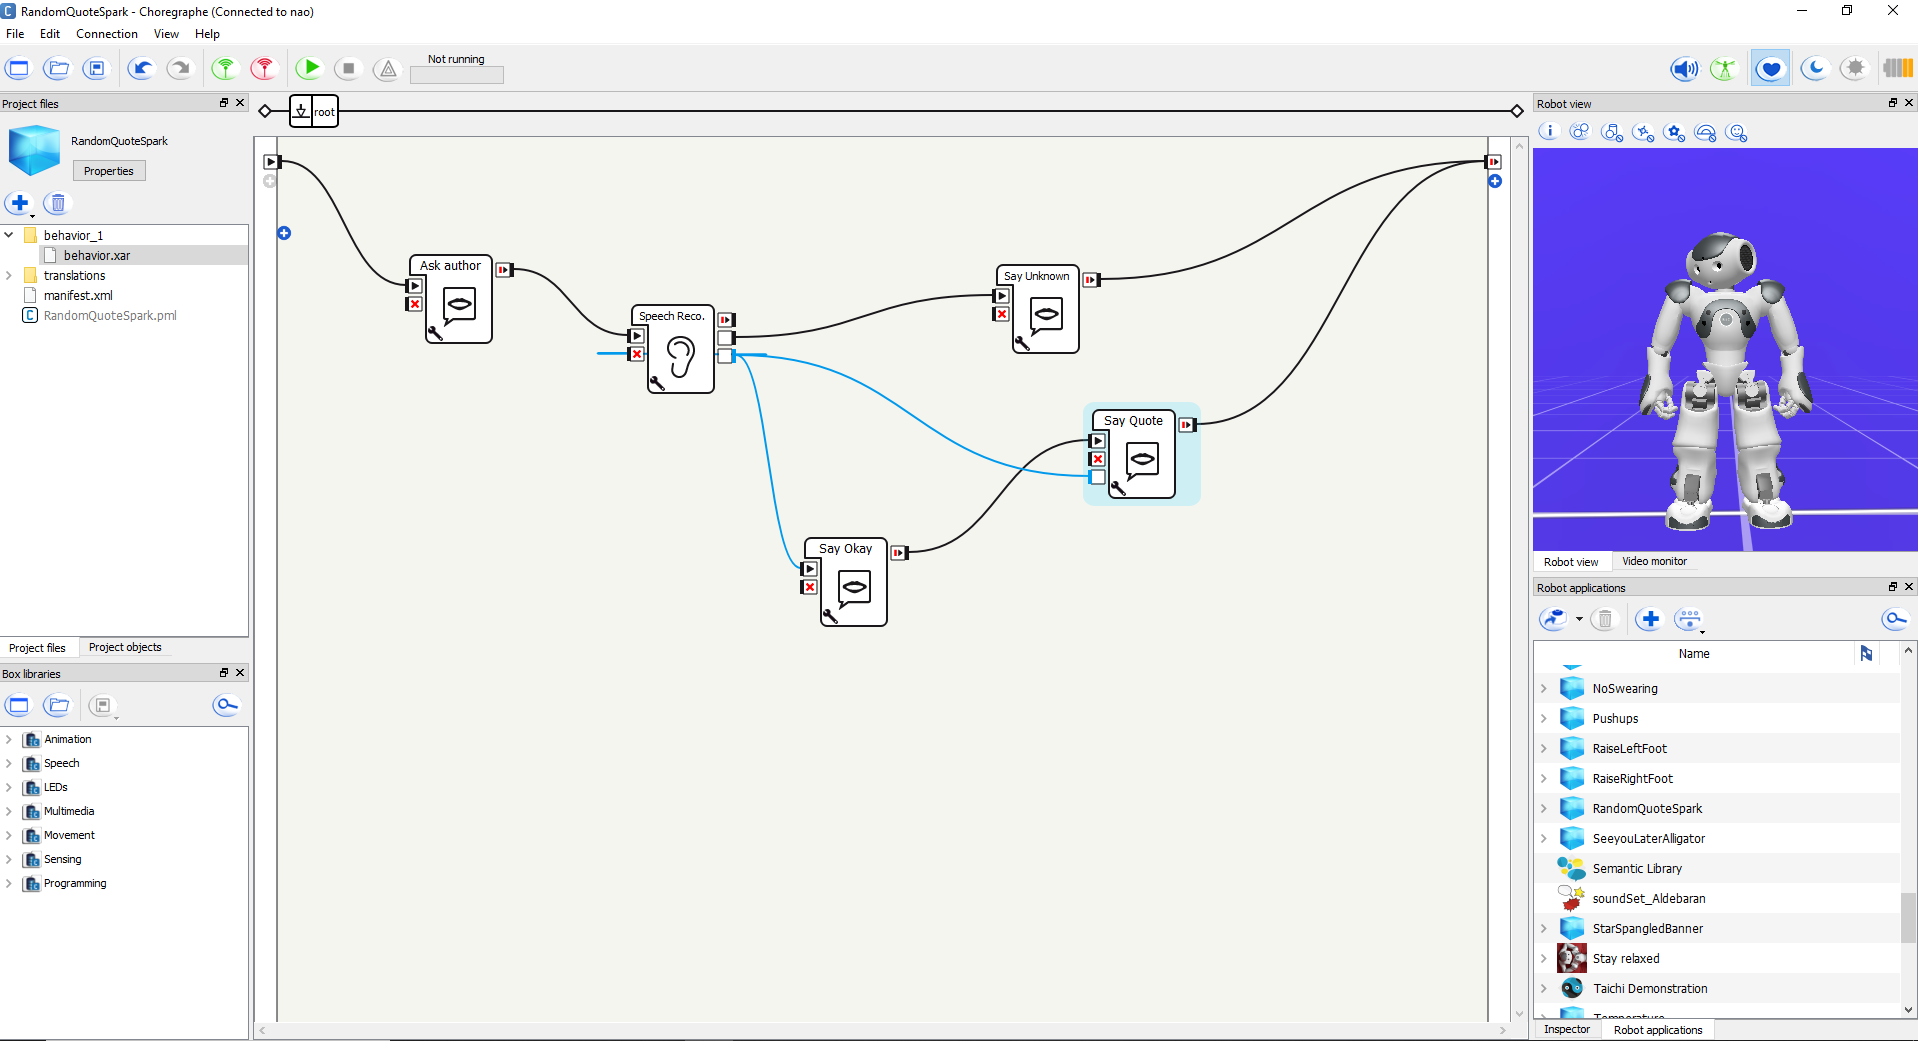
\includegraphics[width =1\linewidth]{robot-spark-proj/screenshot-1.PNG}
    		\caption{Diagram}
    	\end{figure}
    	
    \end{frame}
	{Python2 code with robot}
	\begin{verbatim}
	import time
	import requests
	
	author = ""
	
	class MyClass(GeneratedClass):
	def __init__(self):
	GeneratedClass.__init__(self, False)
	
	def onLoad(self):
	self.tts = self.session().service('ALTextToSpeech')
	self.ttsStop = self.session().service('ALTextToSpeech') #Create another service as wait is blocking if audioout is remote
	self.bIsRunning = False
	self.ids = []
	
	def onUnload(self):
	for id in self.ids:
	try:
	self.ttsStop.stop(id)
	except:
	pass
	while( self.bIsRunning ):
	time.sleep( 0.2 )
	
	def onInput_onStart(self):
	global author
	tts = ALProxy("ALTextToSpeech")
	
	try:
	# Get request from spark webserver
	r = requests.get("http://35.226.85.38:80/?author=" + str(author), timeout=5)
	if r.status_code == 200:
	data = r.json()
	say = ""
	if 'error' in data:
	say = data['error']
	else:
	# Say quote
	say = str(data['quote']) + ". " + str(data['author'])
	
	tts.say(str(say))
	else:
	tts.say("Sorry, I am having trouble accessing the internet right now")
	except requests.exceptions.RequestException as e:
	tts.say(str(e))
	
	self.onStopped() #activate the output of the box
	
	def onInput_authorname(self, p):
	global author
	author = p
	
	def onInput_onStop(self):
	self.onUnload()
	
	\end{verbatim}
    
    \section{Conclusion and References}
    
    \frame{\sectionpage}
    
    \begin{frame}{Conclusion}
         	\begin{itemize}
         	\item This has been a really fun and great learning experience for our group
         	\pause
         	\item Thank you Professor Calvalcanti for great classes and content.
         	\pause
         \end{itemize}
    \end{frame} 
    
    %\section{A Silly Idea}
    
    \frame{\sectionpage}
    
    \begin{frame}{Ordinary Differential Equations}
        \uncover<+->{\begin{equation*}
            \dv{x} y(x) + \frac{1}{CR} y(x) = 0
        \end{equation*}}
        
        \uncover<+->{\begin{equation*}
            \dv[2]{x} y(x) + \gamma \dv{x} y(x) + \omega_0^2 y(x) = f(x)
        \end{equation*}}
    \end{frame}
    
    \begin{frame}{Livin' La Vida Loca}
        \uncover<+>{\begin{equation*}
            \dv[2]{x} y(x) + \gamma \dv{x} y(x) + \omega_0^2 y(x) = f(x)
        \end{equation*}}
        \uncover<+>{\[ \Downarrow \]
        \begin{equation*}
            \colch{\dv[2]{x} + \gamma \dv{x} + \omega_0^2} y(x) = f(x)
        \end{equation*}}
        \uncover<+>{\[ \Downarrow \]
        \begin{equation*}
            y(x) = \frac{f(x)}{\dv[2]{x} + \gamma \dv{x} + \omega_0^2}
        \end{equation*}}
    \end{frame}
    
    \begin{frame}{Livin' La Vida Loca}
        \centering
        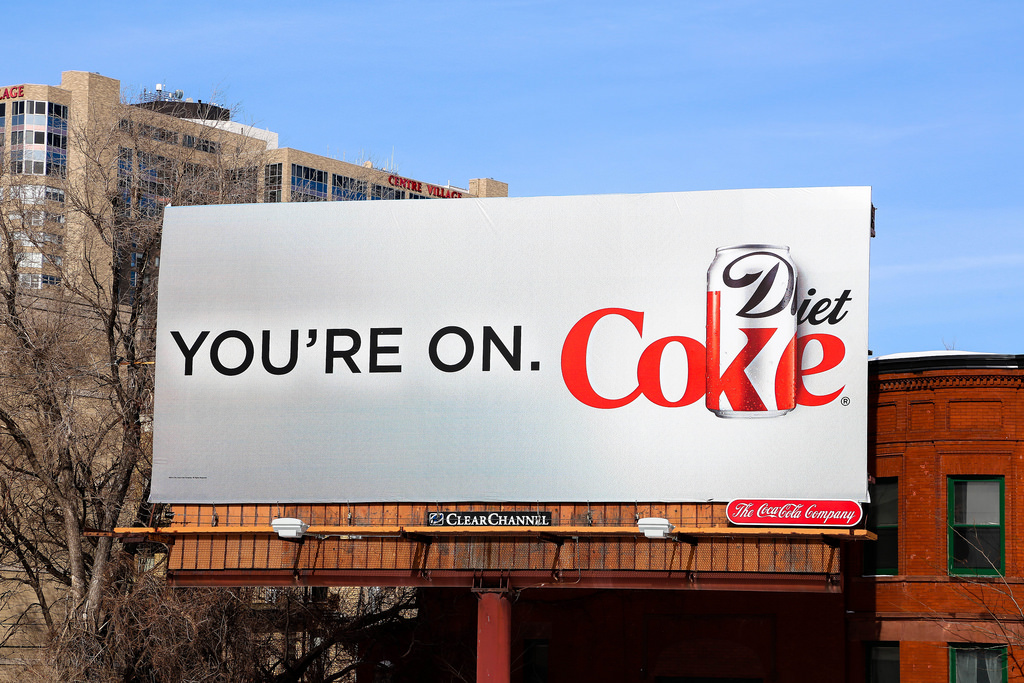
\includegraphics[width = 0.8\textwidth]{images/coke.jpg}
    \end{frame}
    
    \begin{frame}{Pandora's Box}
        \centering
        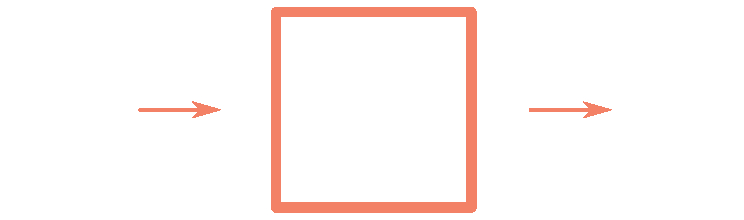
\includegraphics[width = 0.9\textwidth]{images/fourier-1.pdf}
    \end{frame}
    
    \begin{frame}{Pandora's Box}
        \centering
        
\includegraphics[width = 0.9\textwidth]{images/fourier-2.pdf}
    \end{frame}
    
    \begin{frame}{Pandora's Box}
        \centering
        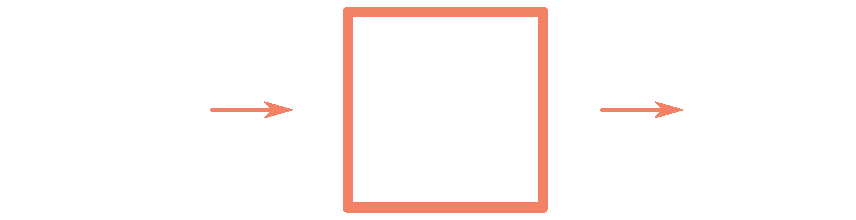
\includegraphics[width = 0.9\textwidth]{images/fourier-3.pdf}
    \end{frame}
    
    \begin{frame}{Pandora's Box}
        \centering
        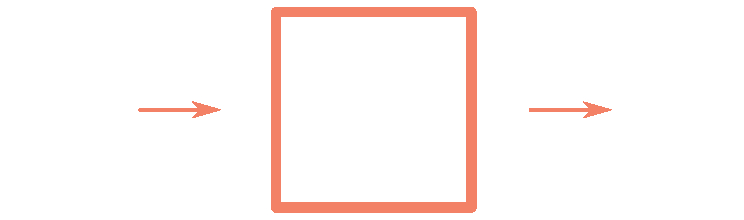
\includegraphics[width = 0.9\textwidth]{images/fourier-4.pdf}
    \end{frame}
    
    \begin{frame}{Pandora's Box}
        \centering
        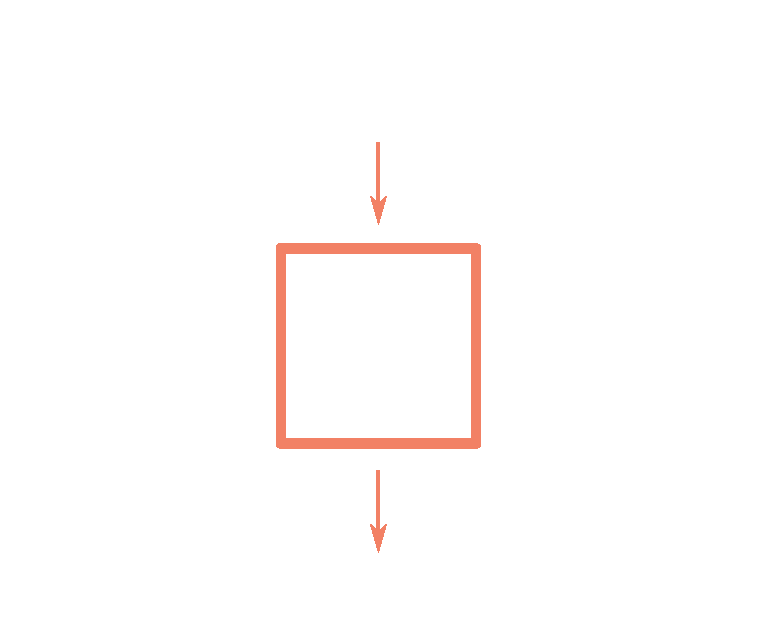
\includegraphics[height = 0.7\textheight]{images/fourier-5.pdf}
    \end{frame}
    
    \begin{frame}{Box Proposal}
        \uncover<+>{\begin{equation*}
            \mathcal{F}[f](\xi) = \hat{f}(\xi) = \frac{1}{\sqrt{2\pi}} \int_{-\infty}^{+\infty} f(x) e^{-i x \xi} \dd{x}
        \end{equation*}}
        \uncover<+>{\begin{equation*}
            \mathcal{F}^{-1}[\hat{f}](x) = f(x) = \frac{1}{\sqrt{2\pi}} \int_{-\infty}^{+\infty} \hat{f}(\xi) e^{i x \xi} \dd{\xi}
        \end{equation*}}
    \end{frame}
    
    \begin{frame}{Quality Control}
        \uncover<+>{\begin{equation*}
            \widehat{(f + \alpha g)}(\xi) = \frac{1}{\sqrt{2\pi}} \int_{-\infty}^{+\infty} \prnt{f(x) + \alpha g(x)} e^{-i x \xi} \dd{x}
        \end{equation*}}
        \uncover<+>{\[ \Downarrow \]
        \begin{equation*}
            \widehat{(f + \alpha g)}(\xi) = \frac{1}{\sqrt{2\pi}} \int_{-\infty}^{+\infty} f(x) e^{-i x \xi} \dd{x} + \frac{\alpha}{\sqrt{2\pi}} \int_{-\infty}^{+\infty} g(x) e^{-i x \xi} \dd{x}
        \end{equation*}}
        \uncover<+>{\[ \Downarrow \]
        \begin{equation*}
            \widehat{(f + \alpha g)}(\xi) = \hat{f}(\xi) + \alpha \hat{g}(\xi)
        \end{equation*}}
    \end{frame}
    
    \begin{frame}{Quality Control}
        \uncover<+>{\begin{equation*}
            \widehat{f'}(\xi) = \frac{1}{\sqrt{2\pi}} \int_{-\infty}^{+\infty} f'(x) e^{-i x \xi} \dd{x}
        \end{equation*}}
        \uncover<+>{\[ \Downarrow \]
        \begin{equation*}
            \widehat{f'}(\xi) = \eval{\frac{f(x) e^{-ix\xi}}{\sqrt{2\pi}}}^{+\infty}_{-\infty} + i\xi \cdot \frac{1}{\sqrt{2\pi}} \int_{-\infty}^{+\infty} f(x) e^{-i x \xi} \dd{x}
        \end{equation*}}
        \uncover<+>{\[ \Downarrow \]
        \begin{equation*}
            \widehat{f'}(\xi) = i\xi \widehat{f}(\xi)
        \end{equation*}}
    \end{frame}
    
    \begin{frame}{Quality Control}
        \centering
        \huge{The inverse does work}
        
        \normalsize{for appropriate functions}
        
        \tiny{and, sometimes, the Fourier Transform of a function is not in the same set as the original function, but let's forget about this since we do not know a decent theory of integration}
    \end{frame} 
    
    %\section{Playing Around With Our New Toy}
    
    \frame{\sectionpage}
    
    \begin{frame}{Fourier Transforming}
        \only<-3>{\uncover<+->{\begin{equation*}
            f(t) = \cos(\omega_0 t)e^{-\pi t^2}
        \end{equation*}}
        \uncover<+->{\begin{equation*}
            \widehat{f}(\omega) = \frac{e^{-\frac{(\omega - \omega_0)^2}{4\pi}} + e^{-\frac{(\omega + \omega_0)^2}{4\pi}}}{2\sqrt{2\pi}}
        \end{equation*}}
        \uncover<+->{\begin{equation*}
            \omega = 2\pi\nu
        \end{equation*}}}
        \only<4>{\begin{equation*}
            f(t) = \cos(2\pi\nu_0 t)e^{-\pi t^2}
        \end{equation*}
        \begin{equation*}
            \widehat{f}(\nu) = \frac{e^{-\pi(\nu - \nu_0)^2} + e^{-\pi(\nu + \nu_0)^2}}{2\sqrt{2\pi}}
        \end{equation*}}
    \end{frame}
    
    \begin{frame}{Fourier Transforming}
        \begin{equation*}
            f(t) = \cos(2\pi\nu_0 t)e^{-\pi t^2}
        \end{equation*}
        \centering
        
        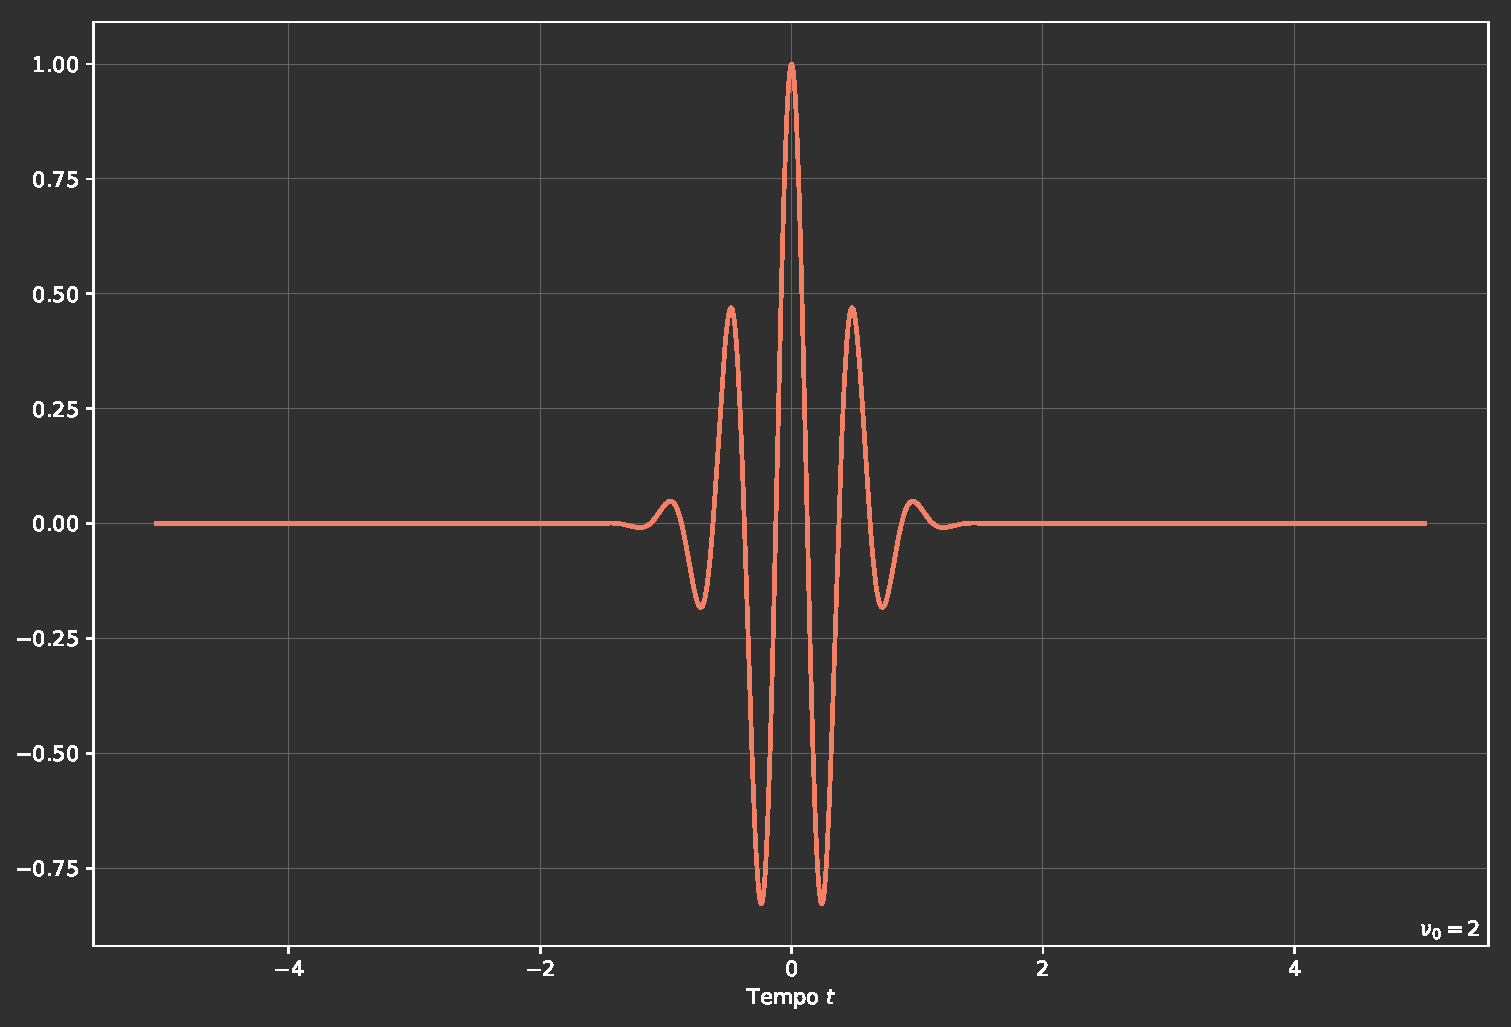
\includegraphics[height = 0.7 \textheight]{images/Pulse1.pdf}
    \end{frame}
    
    \begin{frame}{Fourier Transforming}
        \begin{equation*}
            \widehat{f}(\nu) = \frac{e^{-\pi(\nu - \nu_0)^2} + e^{-\pi(\nu + \nu_0)^2}}{2\sqrt{2\pi}}
        \end{equation*}
        \centering
        
        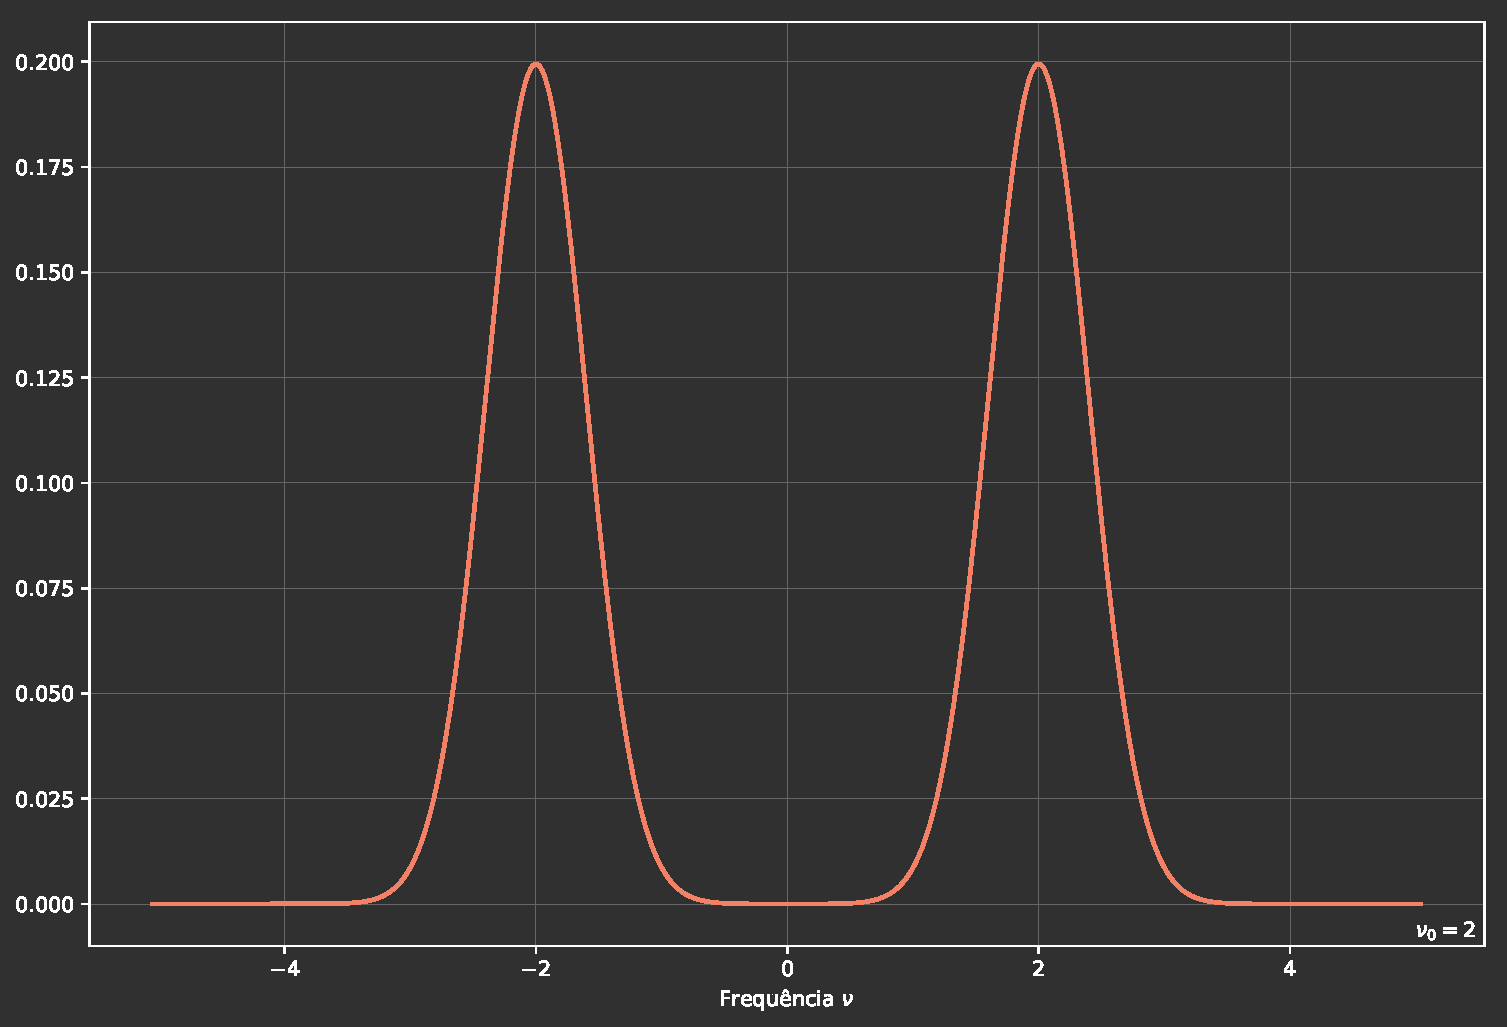
\includegraphics[height = 0.65 \textheight]{images/Pulse1-Fourier.pdf}
    \end{frame}
    
    \begin{frame}{A Harder Example}
        \uncover<+->{\begin{equation*}
            f(t) = e^{i\omega_0 t} = \cos(\omega_0 t) + i \sin(\omega_0 t)
        \end{equation*}}
        \uncover<+->{\begin{equation*}
            \widehat{f}(\omega) = \frac{1}{\sqrt{2\pi}} \int_{-\infty}^{+\infty} e^{i\omega_0 t} e^{-i \omega t} \dd{t}
        \end{equation*}}
    \end{frame}
    
    \begin{frame}{The Mathematical Moonwalk}
        \uncover<+->{\begin{equation*}
            f(t) = e^{i\omega_0 t}
        \end{equation*}}
        \uncover<+->{\begin{equation*}
            e^{i\omega_0 t} = \frac{1}{\sqrt{2\pi}} \int_{-\infty}^{+\infty} \widehat{f}(\omega) e^{i \omega t} \dd{\omega}
        \end{equation*}}
        \uncover<+->{\begin{equation*}
            \widehat{f}(\omega) = \sqrt{2\pi} \dirac{\omega - \omega_0}
        \end{equation*}}
    \end{frame}
    
    \begin{frame}{Cosines}
        \begin{equation*}
            f(t) = \cos(\omega_0 t) = \frac{e^{i\omega_0t} + e^{-i\omega_0t}}{2}
        \end{equation*}
        
        \centering
        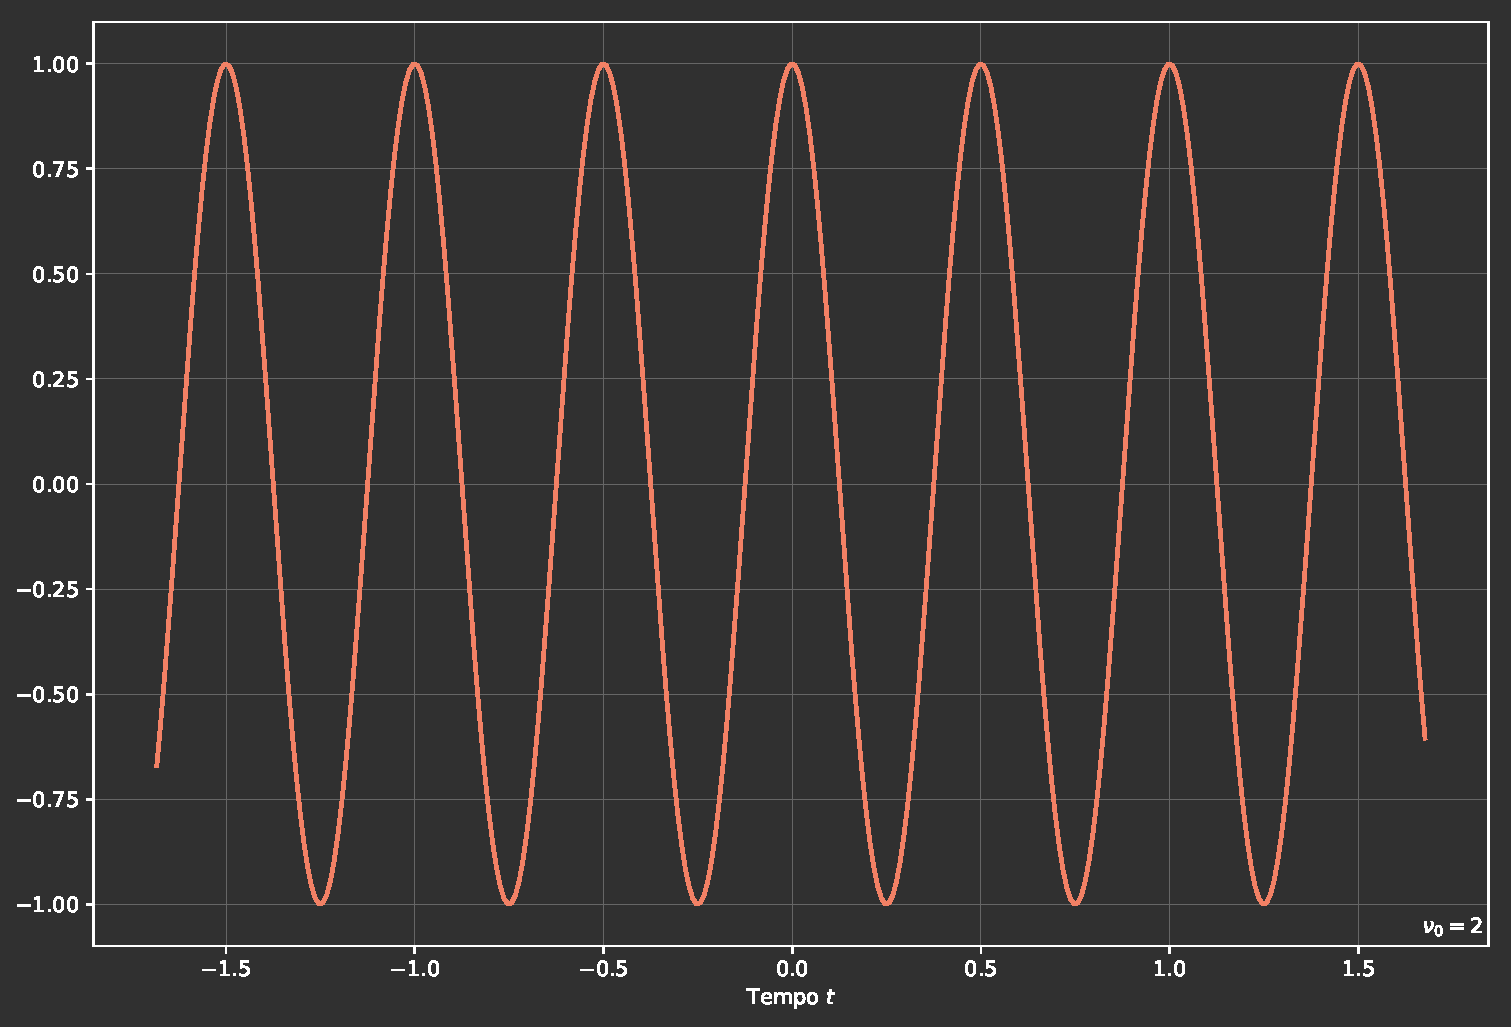
\includegraphics[height = 0.65 \textheight]{images/Pulse2.pdf}
    \end{frame}
    
    \begin{frame}{Cosines}
        \begin{equation*}
            \widehat{f}(\omega) = \sqrt{\frac{\pi}{2}}\prnt{\dirac{\omega-\omega_0} + \dirac{\omega+\omega_0}}    
        \end{equation*}
        
        \centering 
        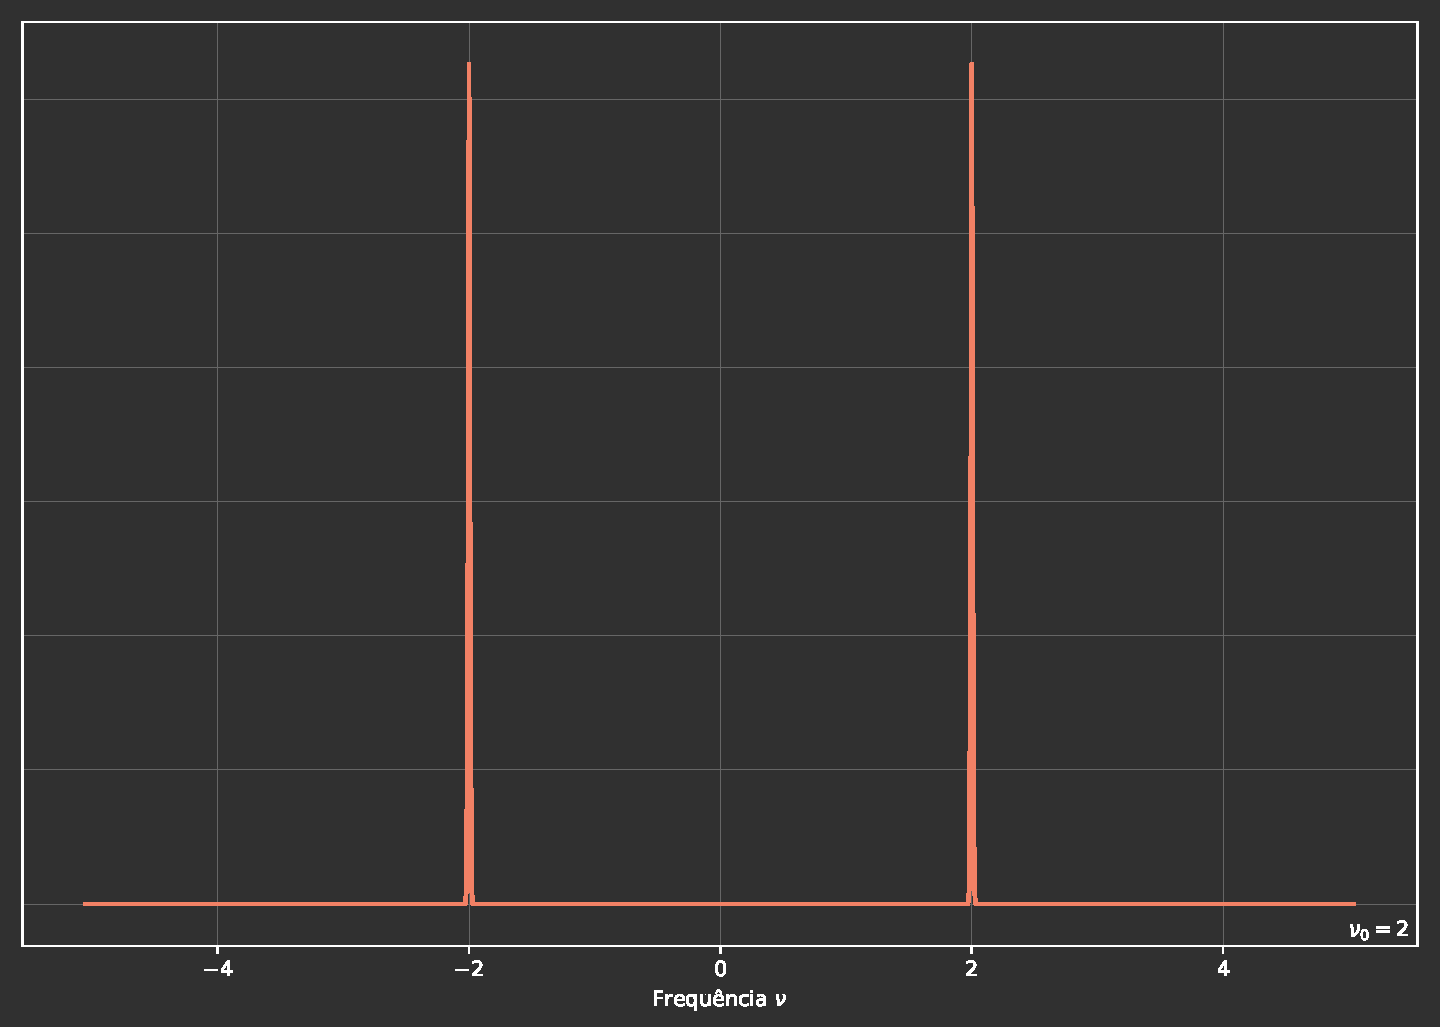
\includegraphics[height = 0.65 \textheight]{images/Pulse2-Fourier.pdf}
    \end{frame}
    
    %\section{Fourier's Physics Playground}

    \subsection{Maxwell's Electrodynamics}
    \frame{\sectionpage}

    \begin{frame}{In the beggining, God said:}
        \begin{equation*}
            \left\lbrace
            \begin{aligned}
                &\div{\vb{E}} = \frac{\rho}{\e}\\
                &\div{\vb{B}} = 0\\
                &\curl{\vb{E}} = - \pdv{\vb{B}}{t}\\
                &\curl{\vb{B}} = \m\vb{J}
 + \m\e\pdv{\vb{E}}{t}                        
            \end{aligned}
            \right.
        \end{equation*}
        
        \uncover<2>{and there was light!}
    \end{frame}
    
    \begin{frame}{Too hard, let's try something different}
        \begin{equation*}
            \left\lbrace
            \begin{aligned}
                &\vb{E} = - \grad{V} - \pdv{\vb{A}}{t} \\
                &\vb{B} = \curl{\vb{A}}
            \end{aligned}
            \right.
        \end{equation*}
    \end{frame}
    
    \begin{frame}{Wave Equations}
        \begin{equation*}
            \left\lbrace
            \begin{aligned}
                &\laplacian{V} - \frac{1}{c^2}\pdv[2]{V}{t} = - \frac{\rho}{\e}\\
                &\laplacian{\vb{A}} - \frac{1}{c^2}\pdv[2]{\vb{A}}{t} = - \m\vb{J}
            \end{aligned}
            \right.
        \end{equation*}
    \end{frame}
    
    \begin{frame}{All Wave Equations In One}
        \begin{equation*}
            \laplacian{\psi(\vb{r},t)} - \frac{1}{c^2}\pdv[2]{\psi}{t} (\vb{r},t) = - g(\vb{r},t)
        \end{equation*}
    \end{frame}
    
    \begin{frame}{Fourier's Opinion}
        \begin{equation*}
            \widehat{g}(\vb{r},\omega) = \frac{1}{\sqrt{2\pi}} \int_{-\infty}^{+\infty} g(\vb{r},t) e^{-i\omega t} \dd{t}
        \end{equation*}
        
        \begin{equation*}
            g(\vb{r},t) = \frac{1}{\sqrt{2\pi}} \int_{-\infty}^{+\infty} \widehat{g}(\vb{r},\omega) e^{i\omega t} \dd{\omega}
        \end{equation*}
    \end{frame}
    
    \begin{frame}{Fourier's Opinion}
        \begin{equation*}
            \widehat{\psi}(\vb{r},\omega) = \frac{1}{\sqrt{2\pi}} \int_{-\infty}^{+\infty} \psi(\vb{r},t) e^{-i\omega t} \dd{t}
        \end{equation*}
        
        \begin{equation*}
            \psi(\vb{r},t) = \frac{1}{\sqrt{2\pi}} \int_{-\infty}^{+\infty} \widehat{\psi}(\vb{r},\omega) e^{i\omega t} \dd{\omega}
        \end{equation*}
    \end{frame}
    
    \begin{frame}{Fourier's Opinion}
        \begin{equation*}
            \laplacian{\psi(\vb{r},t)} - \frac{1}{c^2}\pdv[2]{\psi}{t} (\vb{r},t) = - g(\vb{r},t)
        \end{equation*}
        
        \begin{equation*}
            \laplacian{\widehat{\psi}(\vb{r},\omega)} + \frac{\omega^2}{c^2} \widehat{\psi}(\vb{r},\omega) = - \widehat{g}(\vb{r},\omega)
        \end{equation*}
    \end{frame}
    
    \begin{frame}{Green Function}
        \uncover<+->{\begin{equation*}
            L \phi(\vb{r}) = - s(\vb{r})
        \end{equation*}}
        
        \uncover<+->{\begin{equation*}
            L G(\vb{r} - \vb{r'}) = - \dirac{\vb{r} - \vb{r'}}
        \end{equation*}}
        
        \uncover<+->{\begin{equation*}
            \phi(\vb{r}) = \int G(\vb{r} - \vb{r'}) s(\vb{r'}) \dd{\tau'}
        \end{equation*}}
        
        \uncover<+->{\begin{equation*}
            L \phi(\vb{r}) = \int L G(\vb{r} - \vb{r'}) s(\vb{r'}) \dd{\tau'} =  - \int \dirac{\vb{r} - \vb{r'}} s(\vb{r'}) \dd{\tau'} = -s(\vb{r})
        \end{equation*}}
    \end{frame}
    
    \begin{frame}{One At a Time}
        \uncover<+->{\begin{equation*}
            \laplacian{\widehat{\psi}(\vb{r},\omega)} + \frac{\omega^2}{c^2} \widehat{\psi}(\vb{r},\omega) = - \widehat{g}(\vb{r},\omega)
        \end{equation*}}
        
        \uncover<+->{\begin{equation*}
            \laplacian{G(\vb{r} - \vb{r'})} + \frac{\omega^2}{c^2} G(\vb{r} - \vb{r'}) = - \dirac{\vb{r} - \vb{r'}}
        \end{equation*}}
    \end{frame}
    
    \begin{frame}{Solution for $\vb{r} - \vb{r'} \neq \vb{0}$}
        \uncover<+->{\begin{equation*}
            \frac{1}{r}\dv[2]{(rG)}{r} + k^2 G = 0
        \end{equation*}}
        
        \uncover<+->{\begin{equation*}
            G(r) = \frac{A}{r}e^{\pm i k r}
        \end{equation*}}
    \end{frame}
    
    \begin{frame}{Recovering $0$ Psychological Trauma}
        \uncover<+->{\begin{equation*}
            \laplacian{G(\vb{r} - \vb{r'})} + \frac{\omega^2}{c^2} G(\vb{r} - \vb{r'}) = - \dirac{\vb{r} - \vb{r'}}
        \end{equation*}}
        
        \uncover<+->{\begin{equation*}
            A \int \laplacian{\frac{1}{r}} \dd{\tau'} + 4\pi A \frac{\omega^2}{c^2} \int \frac{r^2}{r} \dd{r}  = - \int \dirac{\vb{r} - \vb{r'}} \dd{\tau'}
        \end{equation*}}
        
        \uncover<+->{\begin{equation*}
            - 4 \pi A  = - 1
        \end{equation*}}
    \end{frame}
    
    \begin{frame}{Back To Our Problem}
        \uncover<+->{\begin{equation*}
            \widehat{\psi}(\vb{r}, \omega) = \int G(\rc)\widehat{g}(\vb{r'}, \omega) \dd{\tau'}
        \end{equation*}}
        
        \uncover<+->{\begin{equation*}
            G(\rc) = \frac{1}{4\pi \rc}e^{\pm i k \rc}
        \end{equation*}}
        
        \uncover<+->{\begin{equation*}
            \widehat{\psi}(\vb{r}, \omega) = \frac{1}{4\pi} \int \frac{\widehat{g}(\vb{r'}, \omega) e^{\pm i k \rc}}{\rc} \dd{\tau'}
        \end{equation*}}
    \end{frame}
    
    \begin{frame}{Actually Solving Our Problem}
        \uncover<+->{\begin{equation*}
            \psi(\vb{r},t) = \frac{1}{\sqrt{2\pi}} \int_{-\infty}^{+\infty} \widehat{\psi}(\vb{r},\omega) e^{i\omega t} \dd{\omega}
        \end{equation*}}
            
        \uncover<+->{\begin{equation*}
            \psi(\vb{r},t) = \frac{1}{4 \pi \sqrt{2\pi}} \iint \frac{\widehat{g}(\vb{r'}, \omega) e^{i \omega t \pm i \omega \frac{\rc}{c}}}{\rc} \dd{\omega} \dd{\tau'}
        \end{equation*}}
    \end{frame}
    
    \begin{frame}{Actually Solving Our Problem}
        \uncover<+->{\begin{equation*}
            \psi(\vb{r},t) = \frac{1}{4 \pi \sqrt{2\pi}} \iint \frac{\widehat{g}(\vb{r'}, \omega) e^{i \omega \prnt{t \pm \frac{\rc}{c}}}}{\rc} \dd{\omega} \dd{\tau'}
        \end{equation*}}
        
        \uncover<+->{\only<-2>{\begin{equation*}
            \psi(\vb{r},t) = \frac{1}{4 \pi} \int \frac{g(\vb{r'}, t \pm \frac{\rc}{c})}{\rc} \dd{\tau'}
        \end{equation*}}
        
        \only<3>{\begin{equation*}
            \psi(\vb{r},t) = \frac{1}{4 \pi} \int \frac{g(\vb{r'}, t - \frac{\rc}{c})}{\rc} \dd{\tau'}
        \end{equation*}}}
    \end{frame}
    
    \begin{frame}{Back at Maxwell's}
        \begin{equation*}
            V(\vb{r},t) = \frac{1}{4 \pi \e} \int \frac{\rho(\vb{r'}, t - \frac{\rc}{c})}{\rc} \dd{\tau'}
        \end{equation*}
        
        \begin{equation*}
            \vb{A}(\vb{r},t) = \frac{\m}{4 \pi} \int \frac{\vb{J}(\vb{r'}, t - \frac{\rc}{c})}{\rc} \dd{\tau'}
        \end{equation*}
    \end{frame}
    
    \begin{frame}{One Last Step} 
        \begin{equation*}
            \left\lbrace
            \begin{aligned}
                &\vb{E} = - \grad{V} - \pdv{\vb{A}}{t} \\
                &\vb{B} = \curl{\vb{A}}
            \end{aligned}
            \right.
        \end{equation*}
    \end{frame}
    
    \begin{frame}{Jefimenko Equations}
        \begin{equation*}
            \vb{E}(\vb{r},t) = \frac{1}{4\pi\e}\int \frac{\hrc}{\rc^2}\rtd{\rho} + \frac{\hrc}{c\rc} \rtd{\pdv{\rho}{t}} - \frac{1}{c^2\rc} \rtd{\pdv{\vb{J}}{t}} \dd{\tau'}
        \end{equation*}
                    
        \begin{equation*}
            \vb{B}(\vb{r},t) = \frac{\m}{4\pi}\int \prnt{\frac{1}{\rc^2} \rtd{\vb{J}} + \frac{1}{c\rc} \rtd{\pdv{\vb{J}}{t}}} \cp \hrc \dd{\tau'}
        \end{equation*}
    \end{frame}
    
    \subsection{Heisenberg's Uncertainty Principle}
    \frame{\sectionpage}
    \begin{frame}{Position and Momentum}
        \uncover<+->{\begin{equation*}
            \psi(x) = \bra{x}\ket{\psi} = \int \bra{x}\ket{k} \bra{k}\ket{\psi} \dd{k} = \frac{1}{\sqrt{2\pi}} \int e^{ikx} \psi(k) \dd{k}
        \end{equation*}}
        
        \uncover<+->{\begin{equation*}
            \psi(k) = \bra{k}\ket{\psi} = \int \bra{k}\ket{x} \bra{x}\ket{\psi} \dd{x} = \frac{1}{\sqrt{2\pi}} \int e^{-ikx} \psi(x) \dd{x}
        \end{equation*}}
    \end{frame}
    
    \begin{frame}{Position and Momentum (but weirder)}
        \uncover<+->{\begin{equation*}
            \left\lbrace
            \begin{aligned}
                &X\ket{\psi} = x \psi(x) \\
                &K \ket{\psi} = - i \pdv{\psi}{x} (x)
            \end{aligned}
            \right.
        \end{equation*}}
        
        \uncover<+->{\begin{equation*}
            \left\lbrace
            \begin{aligned}
                &X\ket{\psi} = - i \pdv{\psi}{k} (k) \\
                &K \ket{\psi} = k \psi(k)
            \end{aligned}
            \right.
        \end{equation*}}
    \end{frame}
    
    \begin{frame}{Fourier Diplomacy}
        \uncover<+->{\begin{equation*}
            \ket{x} \xleftrightarrow[\mathcal{F}^{-1}]{\mathcal{F}} \ket{k}
        \end{equation*}}
    \end{frame}
    
    \begin{frame}{Fourier Uncertainty}
        \begin{enumerate}
            \item<+-> $\psi(x):$ what is $x$?
            \item<+-> $\psi(k):$ what is $k$?
        \end{enumerate}
    \end{frame}
    
    \begin{frame}{Definite Position}
        \begin{equation*}
            \psi(x) = \sqrt{\frac{\pi}{2}}\prnt{\dirac{x-x_0} + \dirac{x+x_0}}    
        \end{equation*}
        
        \centering 
        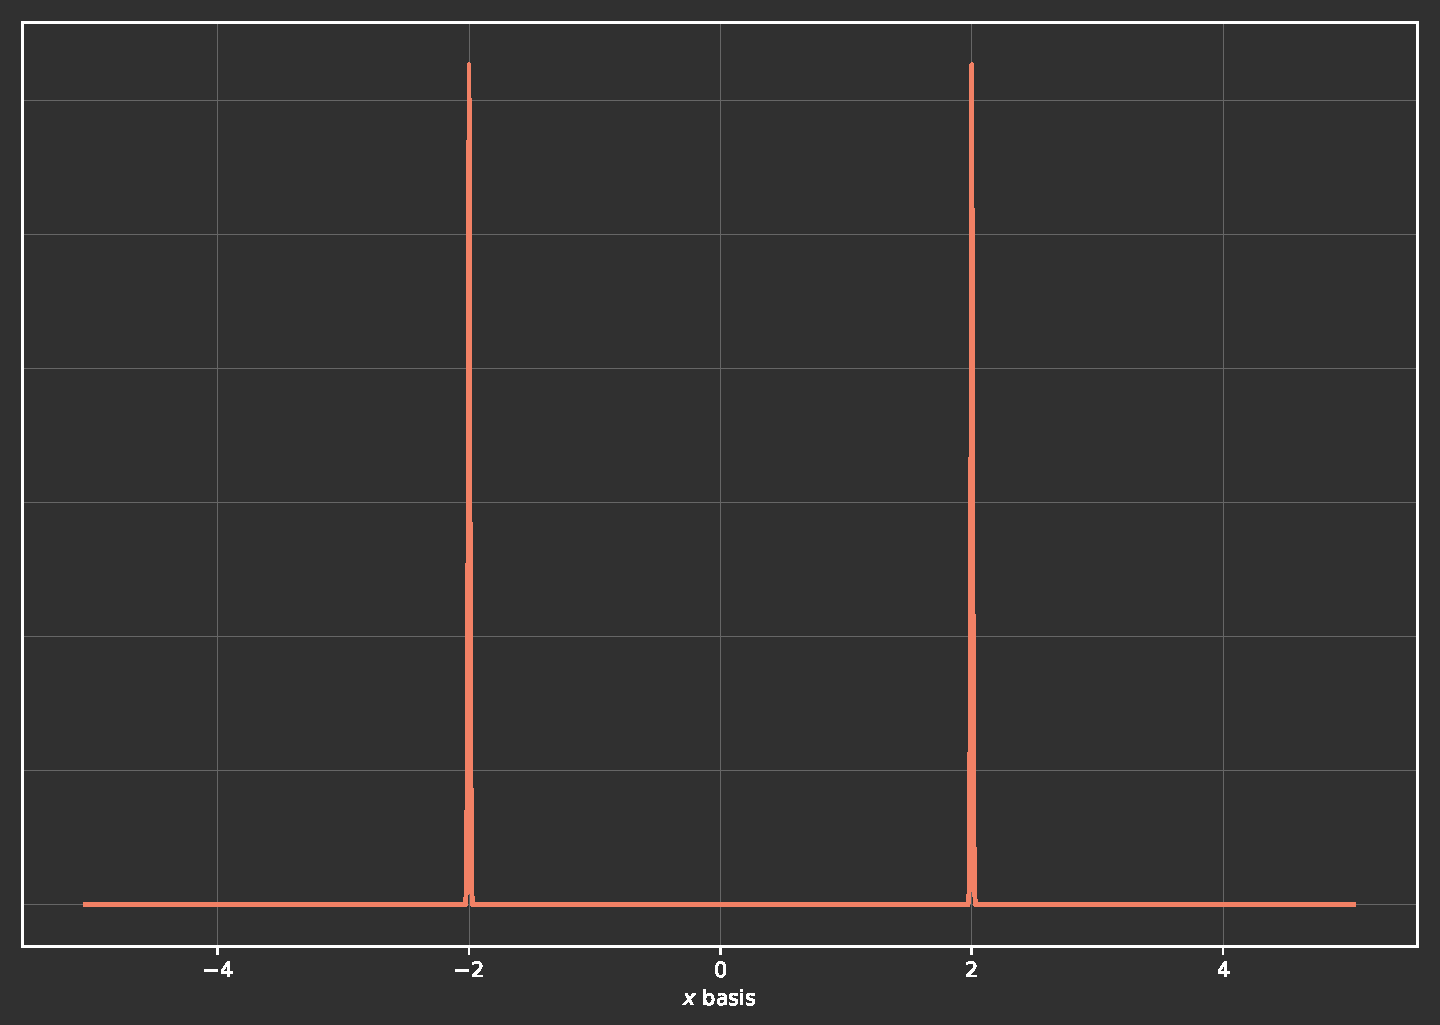
\includegraphics[height = 0.65 \textheight]{images/Pulse3-Fourier.pdf}
    \end{frame}
    
    \begin{frame}{Undefinite Momentum}
        \begin{equation*}
            \psi(k) = \cos(x_0 k) 
        \end{equation*}
        
        \centering
        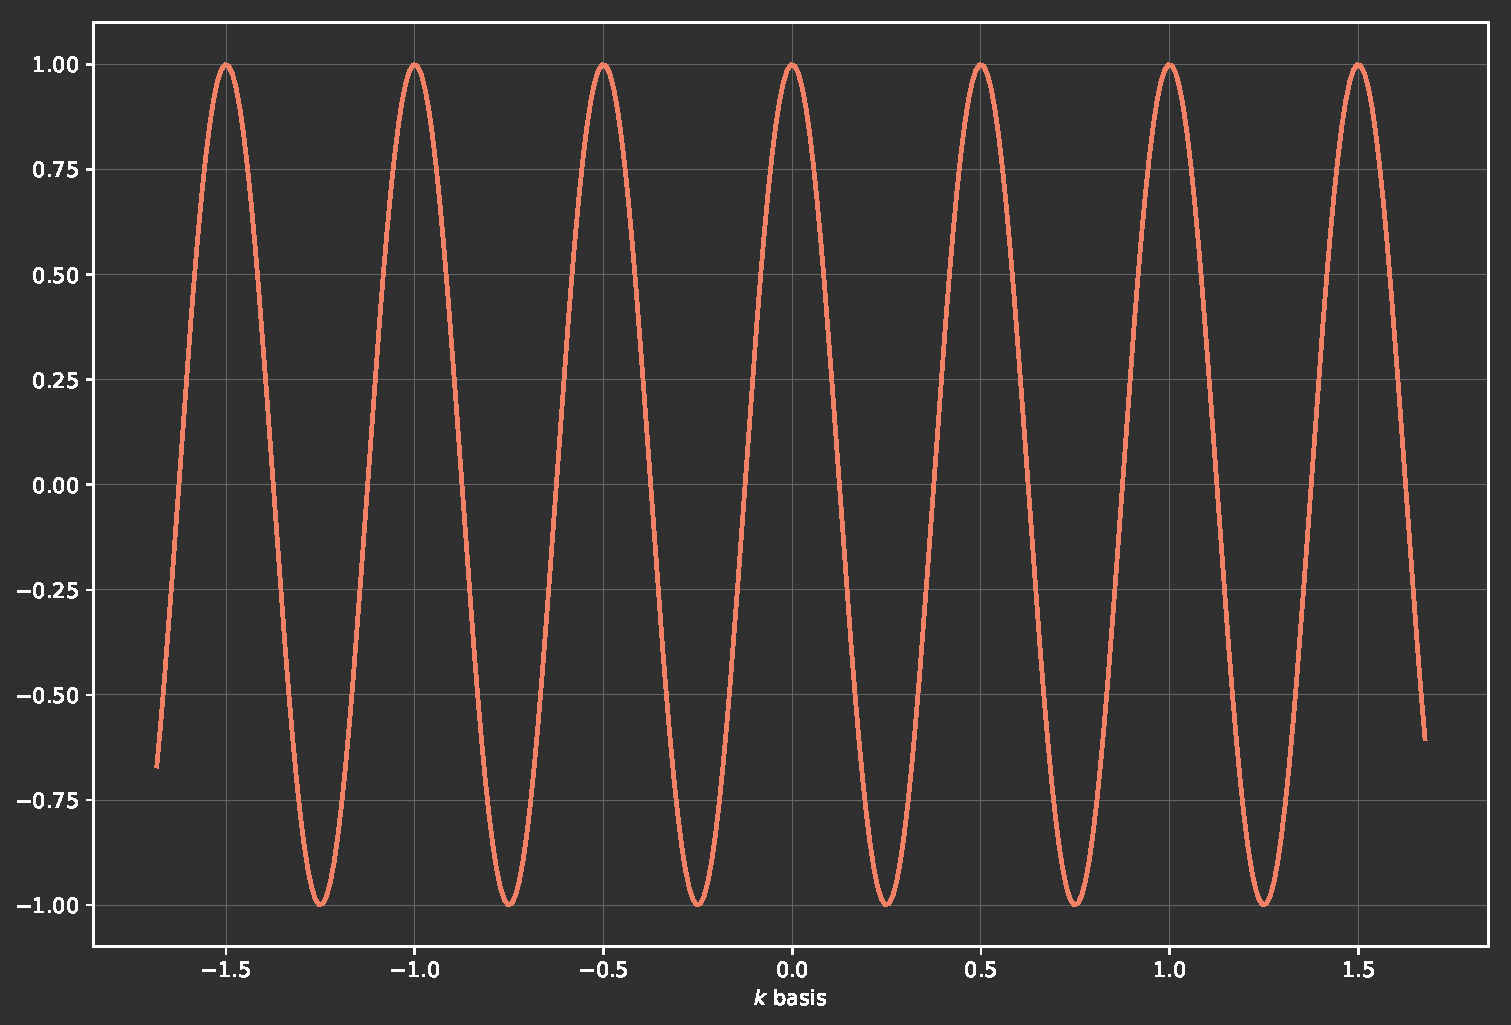
\includegraphics[height = 0.65 \textheight]{images/Pulse3.pdf}
    \end{frame}
    
    \begin{frame}{Uncertainty Relation}
        \begin{block}{\centering$\sigma_x\sigma_p \geq \frac{\hbar}{2}$}
            The uncertainty relation is a consequence of the general fact that anything narrow in one space is wide in the transform space and vice versa. So if you are a 45 kg weakling and are taunted by a 270 kg bully, just ask him to step into momentum space!
        
            \alert{Ramamurti Shankar}
        \end{block}
    \end{frame}
    
%    \section*{Acknowledgments} %You can remove this if you do not want to use it
%        \begin{frame}{Acknowledgments}
%            The author is extremely thankful to Prof. Antônio F. R. T. Piza for the short, yet wonderful, conversations about this seminar.
%        \end{frame}
    
%    \section*{References} %You can remove this if you do not want to use it
%        \nocite{Djairo} \nocite{PhilPanof} \nocite{Fleming} \nocite{Shankar}
%        \begin{frame}{References}
%            \printbibliography
%        \end{frame}

    \section{}
    \begin{frame}{}
        \centering
            \Huge\bfseries
        \textcolor{orange}{The End}
    \end{frame}
\end{document}
